
\section{Are there Grand-Mother Cells in CNNs? How distributed are the representations?}
\label{sec:grand-mother}
 

\cite{GoogleCat} showed the emergence of cat and people specific filters in a deep non-convolutional network. More recently,\cite{DeConv}, \cite{Simonyan} presented visualization methods to find the optimal visual input for a single filter. However, these methods implicitly assumed the presence of single filters which are class specific. This may not be true. Also, visualization methods do not convey the full story. In particular, finding the  optimal visual pattern for a specific filter is akin to maximising,  They are subjective and it is unclear what conclusions may be drawn. Visualizing the tuning of a few filters tells us very little about what the other filters might be doing. To the best of our knowledge there is little work which tries to find an objective answer to this question.

In neuroscience, the presence of neurons  has been hotly debated Most of the above mentioned work can be mathematically treated either as estimating Prob(Filter Activity$\geq$ thresh $|$ Class) or finding the optimal stimulus for a specific unit. We argue that this by itself is an incomplete metric for interpreting how selective a certain filter is. (A hypothetical filter which has the same activation for all classes will score high on this measure.)  The right metric to evaluate if a certain filter is very selective (aka Grand-Mother Cell \cite{Barlow}) is precision defined as Prob(Class $|$Filter Activity $\geq$thresh)

We divide our analysis into two parts. In sec \ref{sub:class-specific-unit} we try to address if there exist filters with very high precision (aka Grand-Mother cells) and in sec \ref{sub:how-many} we answer how many filters are required to discriminate a class. 

\subsection{Are there high precision filters in layer 5?}
\label{sub:class-specific-unit}
Precision for each filter from layer 5 is computed in a way analogous to entropy computation described in \ref{sub:def-ent}. In the final step instead of computing the entropy, we compute Prob(Class $|$ Filter Activity $\geq$ threshold). We define the selectivity of a filter as the area under the precision curve. For this computation we use ground truth bounding boxes taken from PASCAL VOC-2007 test challenge.
From figure \ref{fig:prob-sel} it is clear that for some classes such persons and bicycles there are indeed some very high precision filters, but for a lot of classes like sofa and horses no such filters exist. 

\begin{figure}[t!]
\centering
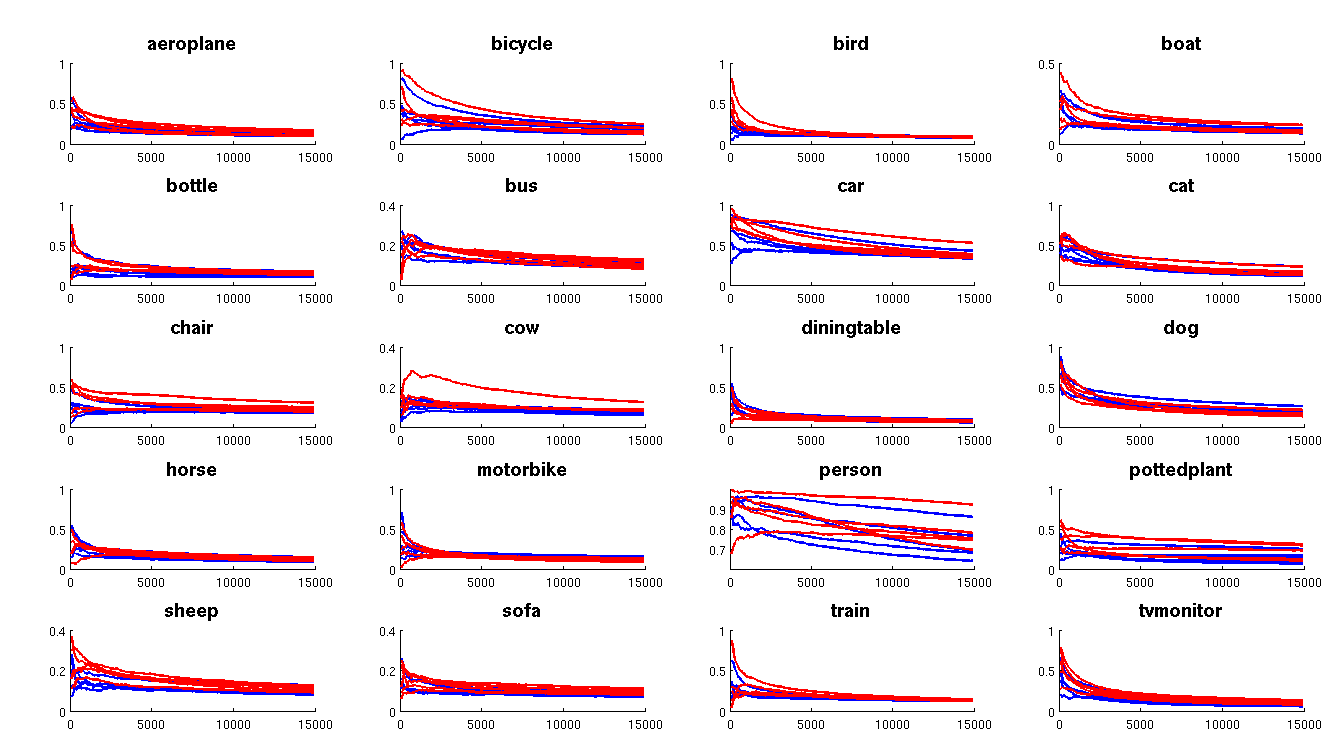
\includegraphics[scale=0.20]{images/prob_sel_dims_top5.png}
\caption{This plot shows the precision curve for the top 5 most selective filters taken from Alex-Net (Blue) and FT-Net(Red) for all PASCAL classes. Y-axis is the precision and X-axis is number of examples.}
\label{fig:prob-sel}
\end{figure}

\subsection{How many filters are required for discrimination?}
\label{sub:how-many}
In order to answer this question we train linear a svm for each class using only a subset of 256 pool-5 filters. In particular we construct subsets of size k, where k takes the values - [1,2,3,5,10,15,20,25,30,35,40,45, \newline 50,80, 100,128,256]. A subset of size k is constructed independently for each class using a greedy selection strategy described in figure \ref{fig:sel-strategy}. We use the variation in performance with the number of filters needed as a metric to evaluate how many filters are needed for each class. 
  
\begin{figure}[t!]
\centering
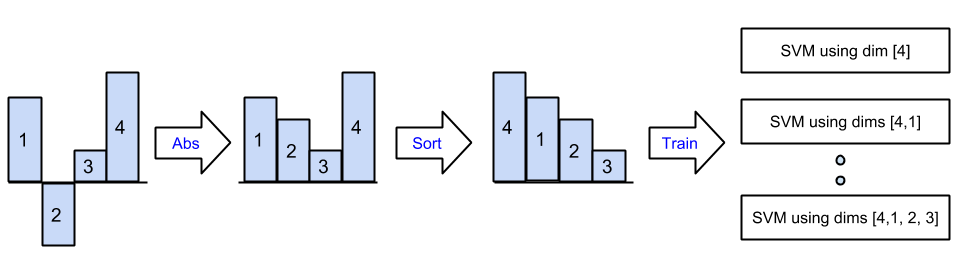
\includegraphics[scale=0.30]{images/how-many.png}
\caption{Illustration of our greedy strategy for constructing subsets of filters. For each class we first train a linear-svm using the spatial-max feature transformation described in section \ref{sub:imp-loc}. Spatial-max leaves us with a 256-D vector wherein each dimension has a one to one correspondence with 256 pool-5 filters. We use the magnitude of each dimension of the learnt weight vector as a proxy for the importance of that dimension towards discriminating a given class. For the purpose of illustration we describe the procedure with a 4-D weight vector shown on the extreme left (the numbers on each bar are the "dimension"). Firstly, we take the absolute value for each dimension and then sort the dimensions based on this value. Then, we chose the top k filters/dimensions from this ranked list to construct a subset of size k.}
\label{fig:sel-strategy}
\end{figure}

The results of our analysis are summarized in fig \ref{fig:svm-sel-dims} and table \ref{table:num-fil}. For classes such as persons, cars, cats we require a relatively few number of filters, but for most of the classes we need to look at around 30-40 filters to achieve atleast 90\% of the full performance. This also indicates, that for a few classes yes, there are grand-mother kind of neurons but for a lot of classes the representation is distributed. Also, as expected the fine-tuned network requires activations of a fewer numbers of filters to achieve the same performance but this reduction in number of filters is not large. 

\begin{figure}[t!]
\centering
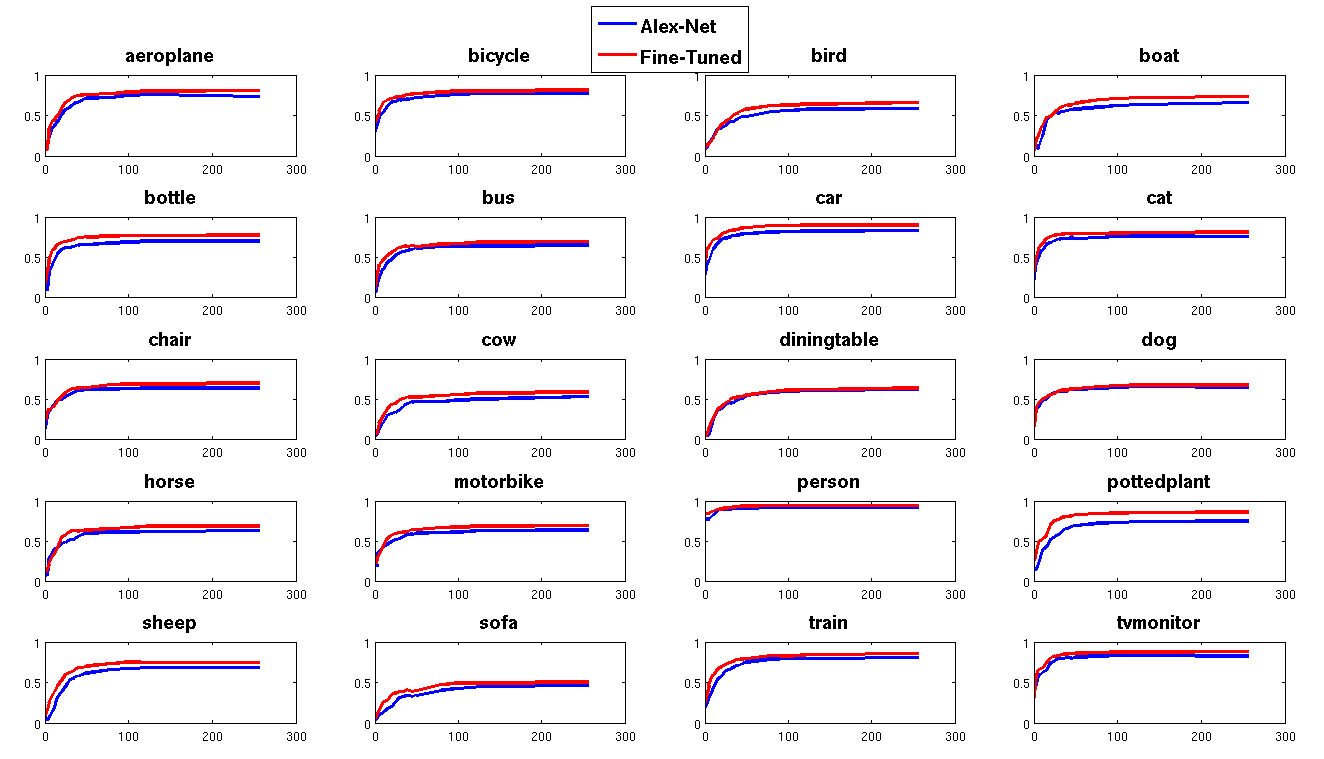
\includegraphics[height=6.5cm]{images/svm_seldims.png}
\caption{Analysis of how many filters are required to classify ground truth bounding boxes for 20 categories taken from PASCAL-2007 detection challenge. The y-axis in each of plot represents classification accuracy measured as mean-ap where as x-axis stand for the number of filters.)}
\label{fig:svm-sel-dims}
\end{figure}



\setlength{\tabcolsep}{1pt}
\begin{table}[t!]
\begin{center}
\caption{Number of filters required to achieve 50\% ,90\% of the full performance for PASCAL classes using Alex-Net(AN) and the Fine-Tuned network(FT)}
\label{table:num-fil}
\tiny
\begin{tabular}{lc||cccccccccccccccccccc}
\hline\noalign{\smallskip}
Net & AP & aero & bike & bird & boat & bottle & bus & car & cat & chair & cow & table & dog & horse & mbike & person & plant & sheep & sofa & train & tv \\
\noalign{\smallskip}
\hline
AN & 50 & 15 & 3 & 15 & 15 & 10 & 10 & 3 & 2 & 5 & 15 & 15 & 2 & 10 & 3 & 1 & 10 & 20 & 25 & 10 & 2 \\ 
FT & 50 & 10 & 1 & 20 & 15 & 5 & 5 & 2 & 2 & 3 & 10 & 15 & 3 & 15 & 10 & 1 & 5 & 15 & 15 & 5 & 2 \\
\hline
\noalign{\smallskip}
AN & 90 & 40 & 35 & 80 & 80 & 35 & 40 & 30 & 20 & 35 & 100 & 80 & 30 & 45 & 40 & 15 & 45 & 50 & 100 & 45 & 25 \\
FT & 90 & 35 & 30 & 80 & 80 & 30 & 35 & 25 & 20 & 35 & 50 & 80 & 35 & 30 & 40 & 10 & 35 & 40 & 80 & 40 & 20 \\
\hline
\end{tabular}
\end{center}
\end{table}
\setlength{\tabcolsep}{1.4pt}

\begin{figure}[t!]
\centering
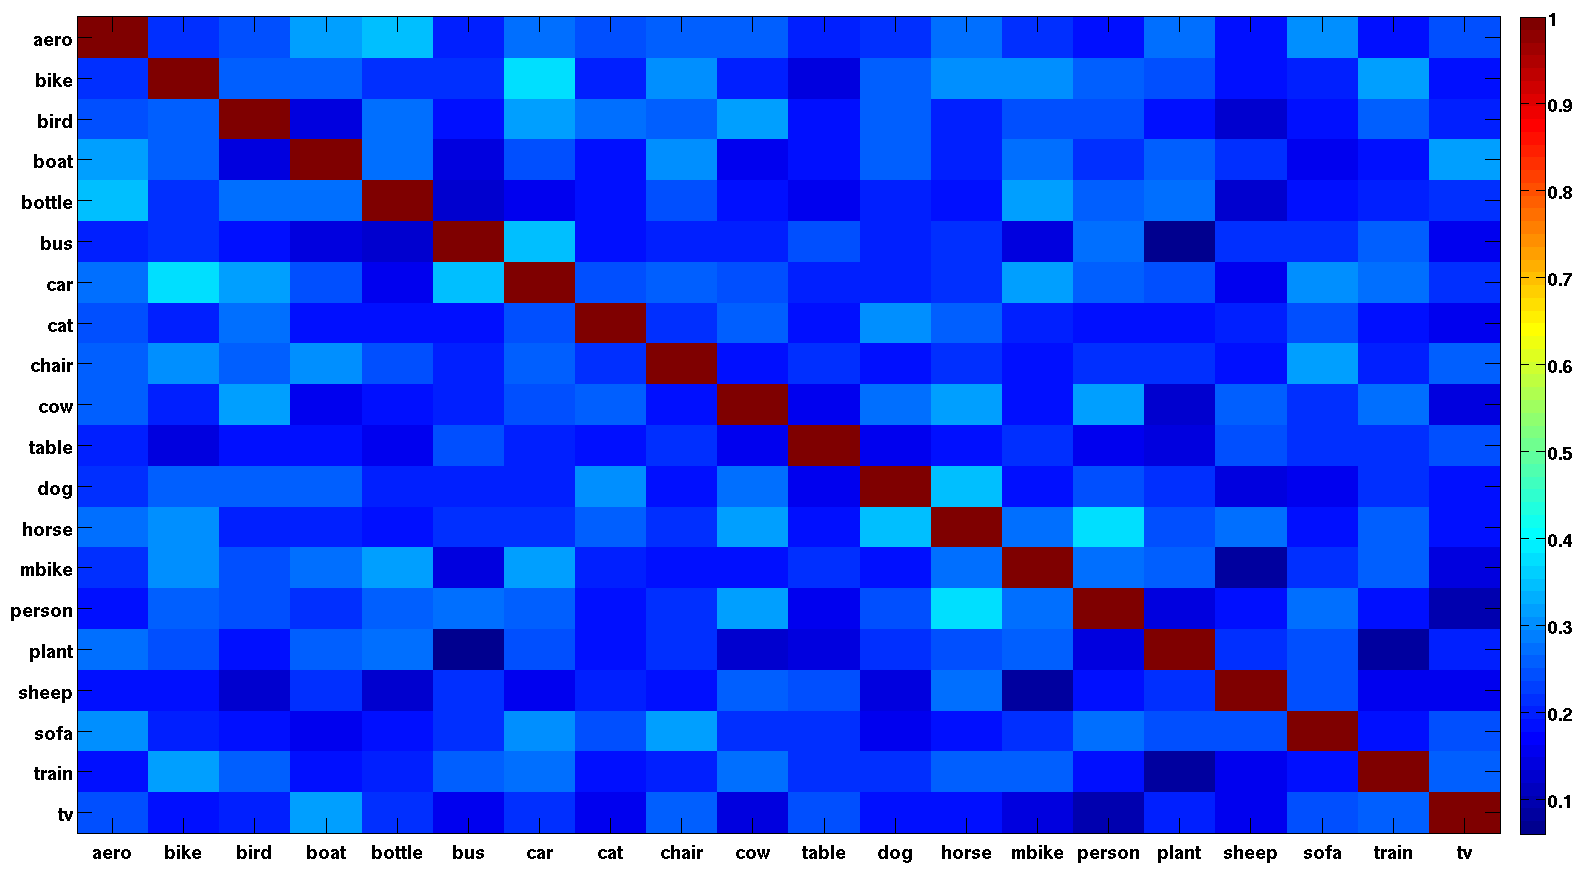
\includegraphics[width=1.0\linewidth]{images/ftNet_commonfilters.png}
\caption{This plot depicts the degree of overlap among the top-50 filters in layer 5 of
finetuned network used for classifying each category of the PASCAL 2007 challenge. Entry
(i,j) of the matrix is the fraction of filters of the i th class which are common with j th class. This plot indicates, that there is very little overlap between filters used for different classes.}
\label{fig:svm-sel-dims}
\end{figure}




\subsection{Discussion}
Although in our analysis we find that for discriminating some classes only a few units suffice whereas for others quite a lot of them are required. The ''extent" to which the code is distributed is likely to be a function of number of filters. If there are a few filters we will expect the code to be more distributed whereas if there are a large number of filters we expect to find more Grandmother kind of cells. The other important tradeoffs to consider are accuracy and training time as a function of number of filters in each layer. We as a community have only had a chance to experiment with a few network architectures out of the exponentially large number of possibilities. Although, it is beyond the scope of the current work determining the optimal number of filters in each layer is an open important question which needs to be addressed! 

